\clearpage

\section{Setup}
\label{sec:setup}

In this section we explain how we set up the experiments with the cluster to see how it performs. We will later list these results and discuss and compare these to results from a MacBook Pro Late 2012.

\subsection{Introduction}
We plan on running these experiments in two phases, first to identify areas where improvement can be made along with bottlenecks and then after attempting to mitigate these to see if any improvement was made, and see where we can end up.

We currently have 3 hardware configurations. The 8 node cluster can be split into:

\begin{enumerate}
\item 1 load distributor and 7 worker nodes
\item 8 worker nodes
\item 5 worker nodes (overclock)
\end{enumerate}

The overclock mode is reduced to 5 workers because the last 3 nodes refused to run properly at the overclocked speed, or didn't boot at all.

In addition we will also look at the i5 MacBook with 1 and 2 threads.

\subsection{Setup}
The setup is the cluster of 8 PI-nodes. Since we are limited by the 8 ports on our switch, we have the load distributor and the load generator connected to another D-Link router that is then connected to the switch.
Also note that we need to be wary of this bottlenecking our total bandwidth to the 7 worker nodes through one cable.
This means we can at most hope to push 100Mbit/s of data to the workers {\em in total}.
The network layout is illustrated in Figure \ref{fig:network}.

\begin{figure}[h]
    \centering
    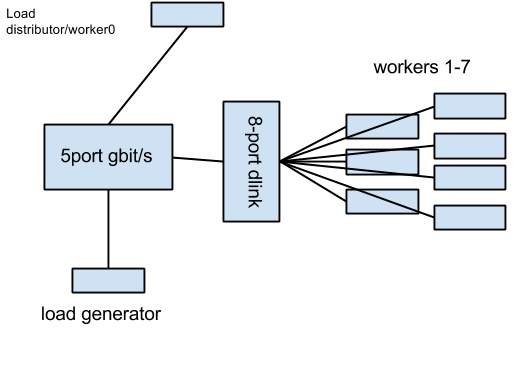
\includegraphics[width=0.8\textwidth]{experiments/networklayout}
    \caption{The network layout for the testing environment.}
    \label{fig:network}
\end{figure}


\subsection{Result gathering}
To obtain results we use a combination of controlling sending, output from the system and measuring the power consumed. To measure power usage we have a COITECH power consumption tool that is placed between the power outlet and our power adapters.
This lets us read the current power consumed by the whole system.

Our load generation utility has a few parameters for us to control. The number of queries to be sent, sending interval, number of threads and the set of nodes to which to send.

\subsection{MacBook Pro control}
When comparing on the MacBook, the load generator is run on a Mac Mini and the search program is run, either in one instance to test single core performance, or in two instances to utilize both the cores.
When running two instances these two operate on different ports.

\clearpage
\section{Results}
\label{sec:experiments}

Here follows our results from the testing.

\subsection{Maximum throughput}
We started out by looking at how many queries we could answer with the cluster, i.e. maximum throughput.

In order to find this we use a load generator which creates random queries and send these at various intervals to the cluster. As the traffic is UDP we expect to see a drop in answers from once the system is over saturated. The load generator is run on a lot more powerful computer outside the cluster.

We do this first by sending queries through a proxy of sorts, the load distributor, which chooses a random worker node to send the query to, then the worker sends the result back to the original client.
Later, we look at exposing direct worker access at the client.

\subsubsection{1 load distributor and 7 workers}
From the numbers in Table \ref{tab:cluster_load_dir} we see that there is a clear drop in performance at around 4400 requests per second. If we increase the load from this point we see a drastic loss in received responses. At this rate the load distributor is running on close to 100\% CPU while the workers are running at around 80\%. So we have reason to believe that the load distributor is holding back the system, effectively being the bottleneck.

\pgfplotstableread{../datasets/cluster_load_dir_requests.txt}\clusterloaddir
\begin{table}[h]
	\centering
	\pgfplotstabletypeset[
     	columns={requests, received},
     	every head row/.style={before row=\hline,
     	after row=\hline},
		every last row/.style={after row=\hline},
		columns/requests/.style={column name=Requests per second},
		columns/received/.style={column name=\% queries served},
     	]
    {\clusterloaddir}
	\caption{Maximum throughput with load distributor}
	\label{tab:cluster_load_dir}
\end{table}

\subsubsection{Required amount of nodes to deliver maximum throughput}
Since the load distributor appears to be a bottleneck in our system, it could be interesting to see how many workers we need to still be able to perform at maximum throughput, i.e. to see how many workers we can drop and still deliver the same amount of work.
In this experiment we have a look at the CPU utilization and query answer rate of the workers while gradually reducing the amount of workers in the cluster.

As suspected, when shutting down nodes one at a time and plotting performance at peak load, we first see an increase in dropped packets after 2 workers have been removed.

The full results are given in Table \ref{tab:clusterreduced}. We see that the cluster could run with 99.7\% of queries answered with 6 instead of 7 workers, and at 97.3\% answered queries with 5. With less than 5 workers, system performance degrades quickly with 78.2\% of queries answered at 4 workers.

We are quite happy with these results as they show that the work distribution looks fairly even. If we only needed a few nodes to handle the maximum throughput from the load distributor, there would be no use for 8 nodes in the cluster.

\pgfplotstableread{../datasets/cluster_reduced_workers_at_full_load.txt}\clusterreduced
\begin{table}
	\centering
	\pgfplotstabletypeset[
     	columns={workers, received},
     	every head row/.style={before row=\hline,
     	after row=\hline},
		every last row/.style={after row=\hline},
		columns/workers/.style={column name=Active working nodes},
		columns/received/.style={column name=\% queries served},
     	]
    {\clusterreduced}
	\caption{Performance when reducing working nodes}
\label{tab:clusterreduced}
\end{table}

\subsubsection{Power usage}
From similar work\cite{RPI_BEOWULF} we have seen that the Raspberry PI will drain up to 15\% more power under heavy load.

\pgfplotstableread{../datasets/watt_per_node.txt}\wattpernode
\begin{table}
	\centering
	\pgfplotstabletypeset[
     	columns={nodes, watt},
     	every head row/.style={before row=\hline,
     	after row=\hline},
		every last row/.style={after row=\hline},
		columns/nodes/.style={column name=Active Nodes},
		columns/watt/.style={column name=Watt},
     	]
    {\wattpernode}
	\caption{Watts consumed under load per node}
    \label{tab:wattpernode}
\end{table}

Despite having read that the Raspberry PIs would drain up to 15\% more energy under load, we were unable to have them drain more than about 9\% more. The cluster runs idle at 22-23W and 23-24W under load. These measurements include the switch which consumes a constant 4W. The power adapter that converts the power for the cluster also has a constant drain of 4W. This leads to the high initial drain we see for the first node.

One source of error for us is that the resolution on the measuring tool is not very high, it does not show decimals, and we do not know how rounding is handled.

\begin{figure}[!h]
\centering
	\begin{tikzpicture}
	\pgfplotstableread{../datasets/watt_per_node.txt}\wattpernode

	\begin{axis}
	[
	xlabel = active nodes,
	xmax = 9,
	xmin = 0,
	ylabel = consumption (W),
	ymax = 30,
	ymin = 0
	]
	\addplot table[y = watt] from \wattpernode ;
	\end{axis}
	\end{tikzpicture}
	\caption{Plot of power drain in the cluster. Shows linear scaling and the fairly high startup cost.}
\end{figure}

\subsubsection{Varying amount of nodes in the cluster}
We also want to vary the amount of nodes that are active in the cluster and plot performance and power consumption to see how it scales.
This is one of the more interesting experiments as one of the strengths of this cluster is that it is easy to power down nodes during hours of low load. We did not get to implement this feature, but it can be done. We will also plot the amount of queries we can deliver per watt used with differing numbers of nodes running.

As we can see from Table \ref{tab:cluster_reqwattnode} we have a steady increase in requests we can service per watt every time we add a node to the cluster. However, since adding any more nodes to the cluster would require a new power supply as well as more network equipment, further scaling would not be very effective, so this is our breakpoint.

\begin{figure}[!h]
\centering
	\begin{tikzpicture}
	\pgfplotstableread{../datasets/cluster_load_dist_request_watt_per_node.txt}\clusterreqwattnode

	\begin{axis}
	[
	xlabel = active nodes,
	xmax = 9,
	xmin = 0,
	ylabel = requests per Watt,
	ymax = 200,
	ymin = 0
	]
	\addplot table[y = reqwatt] from \clusterreqwattnode ;
	\end{axis}
	\end{tikzpicture}
	\caption{Plot showing the }
\end{figure}

\begin{table}
	\pgfplotstableread{../datasets/cluster_load_dist_request_watt_per_node.txt}
	\clusterreqwattnode
	\centering
	\pgfplotstabletypeset[
     	columns={nodes,request,	watt, reqwatt},
     	every head row/.style={before row=\hline,
     	after row=\hline},
		every last row/.style={after row=\hline},
		columns/requests/.style={column name=Requests per second},
		columns/watt/.style={column name=Watt},
		columns/reqwatt/.style={column name=Requests per watt},
     	]
    {\clusterreqwattnode}
	\caption{Efficieny with various nodes}
\label{tab:cluster_reqwattnode}
\end{table}

\subsubsection{Discussion}
After the first phase of testing we can draw some interesting conclusions. With regards to throughput there is a clear point where the system can't keep up with the traffic. At this point the load balancers UDP buffers are filling up and we lose queries.

We verified this by looking at the system network buffers while under load. In Linux, one can look at the buffer status with the command $$netstat -aupn$$, giving something like this:
\begin{lstlisting}[caption={Output of {\tt netstat -aupn | grep 32002}},captionpos=b,label={lst:netstat}]
Proto Recv   Send   Local Addres         Address     PID/name
udp   163840 163840 192.168.0.200:32002  0.0.0.0:*   296/bin/load_distri
\end{lstlisting}
In Listing \ref{lst:netstat} we see that the {\tt Recv} buffer and {\tt Send} buffer are currently containing 163840 bytes.
The maximum size of the buffer is given by {\tt /proc/sys/net/core/rmem\_max}. It is listed in bytes and can be modified with a {\tt sysctl} call: {\tt sysctl -w net.core.rmem\_max=value}.
As we can see in this example, the buffer is currently maxed out, and all additional packages will be lost. The load distributor can not handle any more load. Increasing the buffer size only lead to negligible improvements, as the buffer fills up very quickly.

We also see that the performance quickly diminishes as we increase the load. After the breakpoint, practically no additional queries get answered.
This is to be expected.

Our tests regarding energy consumption and scaling show that there is little difference in a Raspberry PI running idle and full load.
It's also of note that the network switch is at 4 watts responsible for 25\% of the consumed power in the cluster.
This would impact further scaling as it would remove the advantage of each PI improving the efficiency of the cluster.

\subsection{8 workers}
As we discovered in phase 1, the load balancer seems to be limiting the throughput of our cluster.
We therefore try to mitigate this by removing the load distributor entirely and rather have the load generating application (client) deal with distributing work.
This would also make it easier to compare with results of the same system running on the MacBook.

By moving the task of distributing load from the cluster and into the load generator (client library) we of course free up one node in the system, so we now have 8 working nodes for these tests. We expect this to improve our throughput and efficiency by a still linear amount, which we later confirm.

\subsubsection{Maximum throughput phase 2}
As we identified the load distributor as the bottleneck in our system we decided to move the load distribution out into the load generator.
This was implemented by having one thread in the client for each node in the cluster, sending queries at various intervals. The results from the load testing are given in Table \ref{tab:cluster_only_workers}.

\pgfplotstableread{../datasets/cluster_only_workers_requests.txt}\clusteronlyworkers
\begin{table}
	\centering
	\caption{Maximum throughput without load distributor}
	\pgfplotstabletypeset[
     	columns={requests, received},
     	every head row/.style={before row=\hline,
     	after row=\hline},
		every last row/.style={after row=\hline},
		columns/requests/.style={column name=Requests per second},
		columns/received/.style={column name=\% queries served},
     	]
    {\clusteronlyworkers}
\label{tab:cluster_only_workers}
\end{table}

\subsubsection{Scalability and energy efficiency}
As the system still consists of the same nodes doing work we don't expect there to be a change in power consumption, however since there now is 8 workers we should see an improvement in how efficient we can serve queries of various loads.
We will run the same test as in phase 1 where we try to find the breakpoint for the system at an increasing amount of nodes working.

\begin{table}
	\pgfplotstableread{../datasets/cluster_only_workers_request_watt_per_node.txt}
	\clusterworkerreqwatt
	\centering
	\pgfplotstabletypeset[
     	columns={nodes,requests, watt, reqwatt},
     	every head row/.style={before row=\hline,
     	after row=\hline},
		every last row/.style={after row=\hline},
		columns/nodes/.style={column name=Active nodes},
		columns/requests/.style={column name=Requests per second},
		columns/watt/.style={column name=Watt},
		columns/reqwatt/.style={column name=Requests per watt},
     	]
    {\clusterworkerreqwatt}
    \caption{Efficiency with various nodes without load balancer}
\label{tab:cluster_worker_req_watt}
\end{table}

As we can see in Table \ref{tab:cluster_worker_req_watt} we are able to achieve 181 requests per second per watt.
This is an increase of 20\%. This is of course mostly due to having an additional worker pulling its weight, but we are also able to push each individual node harder without the load balancer in place.

\subsubsection{Discussion}
When skipping the load distributor and using only worker nodes we see that it performs better, and a linear increase in performance is indeed observed.
We are now able to service up to around 5000 queries per second. This is an 13\% increase from the 7 workers plus 1 load distributer.
Along with the increase in maximum performance we also see that it behaves a lot better under higher loads.
If we compare the two methods we see that at around 6800 requests per second the load balancer is only able to serve around half its requests, while the cluster is answering 98\% of the requests without the load distributor.

\subsection{Mac VS Cluster of PIs}
In this section we will explore how our system performs compared to a MacBook Pro running the same software. We will again try to find the breakpoints of how much traffic the MacBook can handle and how efficient it can serve the requests. We test in two rounds. First only using 1 search process on the MacBook. This would then not utilize both cores on the CPU. Then we run two processes simultaneously and see how well that performs. We will also measure the power consumption on the mac under both idle and heavy load.

\subsubsection{Maximum throughput}
Running with one core we found the maximum throughput to at around 11000 requests per second. Over double the amount that of the cluster.
However this was to be expected with so much more powerful hardware. With two processes running we were able to push it up to 12700 requests per second. At this point we are pushing the limits of what both the network and the MacBook can handle.

\subsubsection{Energy}
Unlike the Raspberry PIs the MacBook really has a lot of power management built into it. We have measured it running idle at around 18 Watts and managed to push it up to 28 Watts while serving requests.
We also see that how many requests we send to it reflect in the amount of power it consumes. The results of this test can be found in Table \ref{tab:mac_energy_1core} and Table \ref{tab:mac_energy_2core}.

\begin{table}
	\pgfplotstableread{../datasets/mac_energy_1core.txt}
	\macenenrgyonecore
	\centering
	\pgfplotstabletypeset[
     	columns={requests, watt, reqwatt},
     	every head row/.style={before row=\hline,
     	after row=\hline},
		every last row/.style={after row=\hline},
		columns/requests/.style={column name=Requests per second},
		columns/watt/.style={column name=Watt},
		columns/reqwatt/.style={column name=Requests per watt},
     	]
    {\macenenrgyonecore}
    \caption{Mac efficiency 1 core}
\label{tab:mac_energy_1core}
\end{table}

\begin{table}
	\pgfplotstableread{../datasets/mac_energy_2core.txt}
	\macenergytwocore
	\centering
	\pgfplotstabletypeset[
     	columns={requests, watt, reqwatt},
     	every head row/.style={before row=\hline,
     	after row=\hline},
		every last row/.style={after row=\hline},
		columns/requests/.style={column name=Requests per second},
		columns/watt/.style={column name=Watt},
		columns/reqwatt/.style={column name=Requests per watt},
     	]
    {\macenergytwocore}
    \caption{Mac efficiency 2 core}
\label{tab:mac_energy_2core}
\end{table}

It is apparent that under maximum load not surprisingly there is no way the PI Cluster can contest the MacBook Pro other price.
However it is interesting to see how our system compares on lower request rates compared to the MacBook.
Request rates that are within the limits of our system, the system surprisingly performs comparable to the MacBook.

\subsubsection{Cold reads}
While all the other experiments have been performed on the cluster after a significant number of queries already has been answered. This ensured replicate-able results as we assume most the query words are already in memory and cache. However it would be interesting to see how the two compares when answering queries right after a reboot. In this experiment we send 5000 queries to each core operating, so in total 10000 for the MacBook and 40000 for the cluster. We then try pinpoint the breakpoint where the machines are unable to keep up with the load. The Pi cluster is run in the mode where all nodes are workers.

When measuring these numbers we ran into some interesting problems. For one, the sleep system call we use to limit the interval between queries is limited at milliseconds. This turned out to be a problem for measuring the performance of the MacBook Pro as its breakpoint lies somewhere between the minimum sleep duration and no sleep duration. This is reflected in table\ref{tab:coldread_mac} where we have a gap between a load we clearly can support and a load we clearly cannot support.

\begin{table}[h]
	\pgfplotstableread{../datasets/coldread_pi.txt}
	\coldreadpi
	\centering
	\pgfplotstabletypeset[
     	columns={nrps, nanswers, orps, oanswers},
     	every head row/.style={after row=\hline},
		every last row/.style={after row=\hline},
		columns/nrps/.style={column name=Rps},
		columns/nanswers/.style={column name=received(\%)},
		columns/orps/.style={column name=Rps(O)},
		columns/oanswers/.style={column name=received(\%)(O))},
     	]
    {\coldreadpi}
    \caption{Cold reads Pi cluster. Requests per second, and answers received in \%. (O) is with code optimization}
\label{tab:coldread_pi}
\end{table}

\begin{table}[h]
	\pgfplotstableread{../datasets/coldread_mac.txt}
	\coldreadmac
	\centering

	\pgfplotstabletypeset[
     	columns={nrps, nanswers, orps, oanswers},
     	every head row/.style={after row=\hline},
		every last row/.style={after row=\hline},
		columns/nrps/.style={column name=Rps},
		columns/nanswers/.style={column name=received(\%)},
		columns/orps/.style={column name=Rps(O)},
		columns/oanswers/.style={column name=received(\%)(O)},
     	]
    {\coldreadmac}
    \caption{Cold reads MacBook. Requests per second, and answers received in \%. (O) is with code optimization}
\label{tab:coldread_mac}
\end{table}

Without optimization the Pi cluster is able to support around 3000 requests per second. This is 60\% of the load it could handle previously. We also see that the code optimization does increase this number to 80\%.

The Macbook fared similarly. At only around 5500 rps the performance is halved. With the optimization the performance is somewhere between 7000 and 10000.

We did expect the cluster to gain some ground when we forced this much disk access. However as the MacBook runs on flash storage with reading speeds of up to 400MB/s and the poor Pis have SD-cards providing 5-8MB/s, the MacBook does have an unfair advantage.

\section{Overclocking}
Over clocking is the process of making a computer operate at a faster clock rate than the manufacturer intended. This is done by changing software parameters, typically by increasing the operating voltage. Side effects of this process is an increase in power consumption and heat dissipation.

As every operation in our system is bounded by CPU speed, it would be reasonable to expect enhanced performance by over clocking the CPU. The Raspberry PI is very simple to over clock. By editing boot config-file one can easily change the CPU parameters.

This file can be found under:

\begin{lstlisting}
\boot\config.txt
\end{lstlisting}

\begin{lstlisting}
## Some over clocking settings, govenor already set to on demand

##None
#arm_freq=700
#core_freq=250
#sdram_freq=400
#over_voltage=0

##Modest
#arm_freq=800
#core_freq=300
#sdram_freq=400
#over_voltage=0

##High
#arm_freq=950
#core_freq=450
#sdram_freq=450
#over_voltage=6

##Turbo
arm_freq=1000
core_freq=500
sdram_freq=600
over_voltage=6
\end{lstlisting}

By changing from no over clocking to turbo mode we increase the clock frequency from 700MHz to 1000MHz. We also increase the GPU core frequency which drives the L2 cache.

As mentioned in the hardware section, overclocking the Raspberry PI might bring certain downsides. Users have experienced data corruption on the SD card as well as general instability. There are also reports of different degrees of tolerance among the Raspberry PIs. Some works perfectly under any degree of overclocking while others quickly start showing symptoms of instability.

We started out by overclocking one node and then run some tests. Everything seemed to work, so we added the overclocking parameters to the entire cluster. After then rebooting the cluster we experienced all the problems mentioned above. One node had problems with its SD-card and two others were struggling with booting or network access. We did however manage to find a stable set of five nodes to compare with our existing results. In this experiment we ran five individual workers similarly to when we tried to pin point the maximum performance of the cluster with various amounts of nodes.

We were able to see an increase in throughput of around 10\% with the cores overclocked. This number was a lot lower than expected taking into account that the cluster was using 21 watts compared to 16 without the overclock. At this rate the cluster can deliver 133 requests per watt, compared to 152 without the overclock. So this was generally bad value.


\section{Further optimization}
In an attempt to further improve our performance we have tried some optimization in our code. One of them being changing the load distributor from using $$rand() \bmod N,$$ where N is the number of nodes in the cluster, to just keeping iterating over the range 1-7 instead. We did however not notice any change from that.

Originally we always sent queries as 1024 byte messages. This was done for simplicity but of course at a cost of performance. By instead sending only as many bytes as needed we saw a dramatic increase in performance. Doing all measurements again was not an option but we did measure some values for comparison again.

















